\section{Mixtures beat the best Gaussian state}
\label{sec:mixtures}

Since Gaussian states are often extremal for information inequalities~\cite{stam1959,cover2006}, it is natural to ask whether $R \leq R^*(\sigma)$ for every state. It is not. We measure the advantage of a state over the best Gaussian state at the same resolution, in units of the Gaussian gap, by
\begin{equation}
g^* = \frac{R - R^*(\sigma)}{1 - R^*(\sigma)} .
\label{eq:gstar}
\end{equation}

\begin{observation}[Fans of segments]
\label{obs:fan}
For the pendulum there are Gaussian mixtures with $g^* > 0$ at every $\sigma$ examined ($10^{-5} \leq \sigma \leq 0.3$). Adversarial searches found $g^* = 0.031$, $0.037$ and $0.043$ for $K = 2, 3, 4$ components at $\sigma = 10^{-3}$, and $g^* = 0.053$ for $K = 8$. The optimal states are fans of thin segments that all pass through the hyperbolic point $q = \pi$, with slightly different tilts and lengths (Fig.~\ref{fig:fan}). A fan described by continuous profiles of weight, length, thickness and offset over the tilt angle reaches $g^* = 0.0478$, unchanged between $20$ and $80$ segments. The advantage is scale invariant: rescaling a state from $\sigma = 10^{-3}$ to $10^{-5}$ changes $g^*$ by less than $2\times10^{-3}$. In every case $R < 1$. For $\sigma \leq 10^{-2}$ the gap satisfies $(1-R)/\sigma \geq 0.946$; at larger $\sigma$ the gaps of all states, including the best Gaussian one, fall below $\sigma$ through the higher-order terms of Eq.~\eqref{eq:series}, and the advantage of mixtures stays at a few percent of the Gaussian gap (Fig.~\ref{fig:fan}, panel 3).
\end{observation}

The violation of $R \leq R^*$ was confirmed by three independent evaluations: closed-form posterior moments with quadrature on four grids, Gauss--Hermite quadrature of the posterior expectations, and a direct summation over nodes of the fine-grained state that uses no closed forms. In addition, the coarse-grained entropy was computed directly on a grid and differentiated in time, without using any of the identities of Sec.~\ref{sec:decomposition}; for two of the violating states ($\sigma = 0.1$ and $0.3$) this reproduced $R - R^* = 0.002390$ and $0.005528$ to $10^{-7}$ (Appendix~\ref{app:methods}).

The mechanism is visible in the decomposition~\eqref{eq:decomposition}. Each component of the fan is, on its own, below the best Gaussian state. In the mixture the components overlap only near the common point $q = \pi$, so the focus of the coarse-grained density concentrates where the strain is maximal. A single segment spreads its focus uniformly over its length and cannot do this. The gain comes from the covariance term $C$; the Stein defect is negligible ($D \approx 3\times10^{-7}$ for the best $K = 4$ state).

\begin{figure*}[t]
\centering
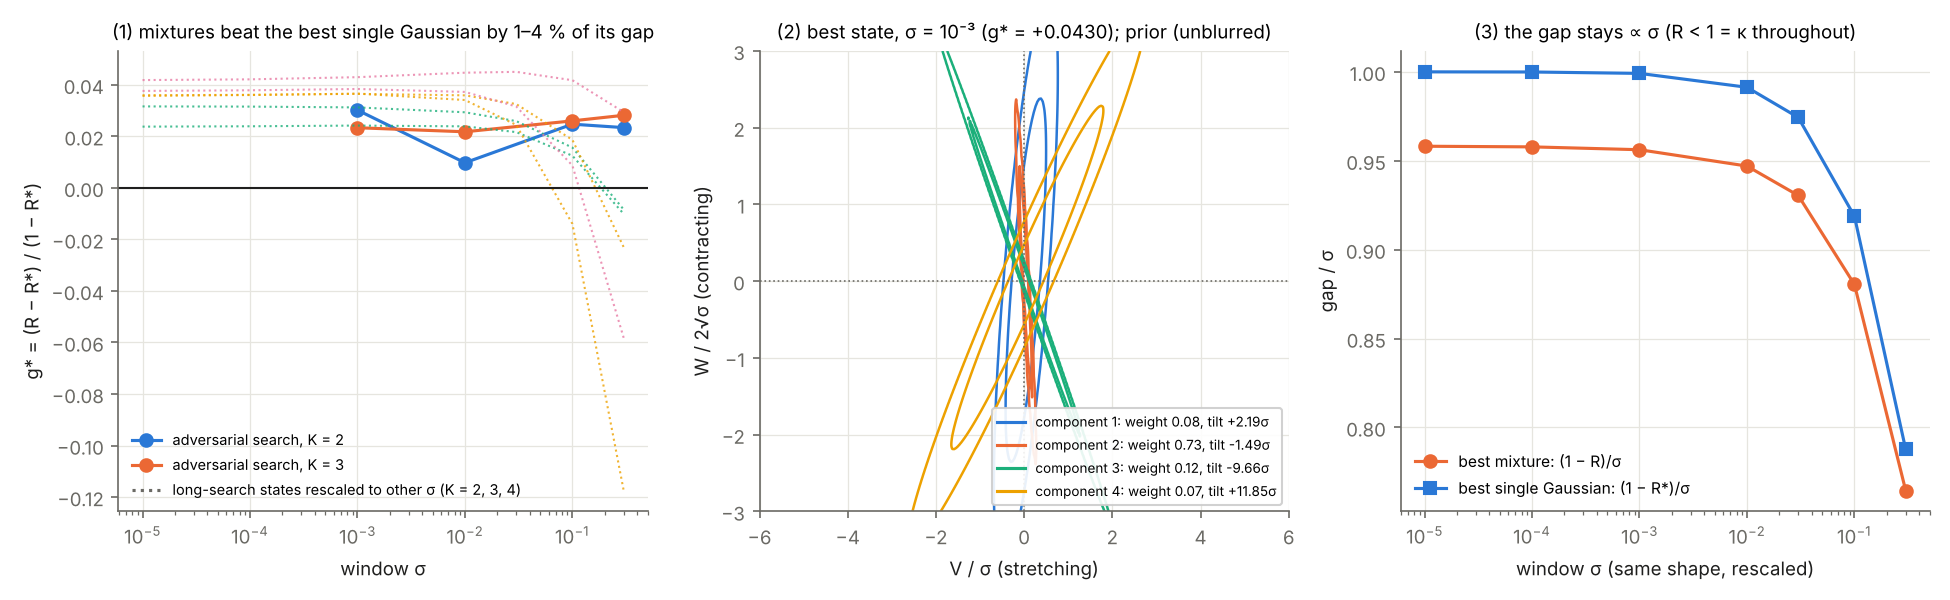
\includegraphics[width=0.95\textwidth]{figures/fig3_fan.png}
\caption{Mixtures that beat the best Gaussian state (pendulum). (1) Advantage $g^*$ of adversarially optimized mixtures with $K = 2$ and $3$ components, and of long searches rescaled to other $\sigma$. (2) The best state at $\sigma = 10^{-3}$ ($K = 4$): four thin components crossing at $q = \pi$, shown in units of $\sigma$ across and $2\sqrt\sigma$ along. (3) The gap stays proportional to $\sigma$ for the best mixture and for the best Gaussian state.}
\label{fig:fan}
\end{figure*}

In the twist flow, where the stretching direction rotates, the advantage is much larger.

\begin{observation}[Bent needles]
\label{obs:bent}
For the twist flow $H = \tfrac12\ln(1+q^2+p^2)$, $\kappa = 1/4$, the best Gaussian state has gap $(\kappa - R^*)/\sigma \to \sqrt3/2 \approx 0.866$. Mixtures reach $0.525$ ($K = 8$), and a needle bent along an arc reaches $0.509$. The optimal curvature, $0.709$ to $0.714$ in four independent optimizations, equals the rate $1/\sqrt2$ at which the stretching direction turns along the contracting direction, and the gap agrees with $2\sqrt{2\beta_{\rm eff}\kappa} = 1/2$ for $\beta_{\rm eff} = 1/8$, the value of $\beta$ without the turning contribution. The gap is scale invariant ($\sigma = 10^{-4}$ to $10^{-2}$) and remains proportional to $\sigma$.
\end{observation}

We reproduced the gap of the best $K = 8$ twist state by a direct summation over nodes of each component, transported by the exact flow, with the entropy computed on a grid and differentiated in time: $R = 0.24946085749$ against $0.24946085792$ from the closed-form evaluator.

The bent needle shows that a state can follow a rotating frame of stretching directions and so remove the part of $\beta$ that comes from the rotation. What cannot be removed is the decrease of the strain itself away from its maximum, which is why the gap stays linear in $\sigma$. For the double well and the quartic oscillator, where the stretching direction is fixed, short searches found only small advantages ($g^* \leq 0.02$), comparable to the pendulum fan.
